%%TC:ignore
\section{Programming Languages}
\label{sec:appendix-programming-languages-comparison}

In terms of speed, compiled languages are quicker than interpreted languages, but because the main bottleneck in a deep learning system is the training phase of the model, which mainly relies on the library used rather than the language itself, speed is not taken into account. 

\begin{table}[h]
\centering
\resizebox{\textwidth}{!}{%
\begin{tabular}{l|l|l|l|l|}
\cline{2-5}
\multicolumn{1}{c|}{} &
  \multicolumn{1}{c|}{\textbf{Python}} &
  \multicolumn{1}{c|}{\textbf{Java}} &
  \multicolumn{1}{c|}{\textbf{R}} &
  \multicolumn{1}{c|}{\textbf{Javascript}} \\ \hline
\multicolumn{1}{|l|}{\textbf{Familiarity}} &
  Extremely familiar &
  Familiar &
  Unfamiliar &
  Familiar \\ \hline
\multicolumn{1}{|l|}{\textbf{\begin{tabular}[c]{@{}l@{}}Deep Learning \\ Libraries support\end{tabular}}} &
  \begin{tabular}[c]{@{}l@{}}Tensorflow, Keras, \\ PyTorch + ML suite \\ (NumPy, Pandas, \\ MatplotLib, Pandas)\end{tabular} &
  \begin{tabular}[c]{@{}l@{}}DL4J \\ \\ (Deeplearning4j)\end{tabular} &
  \begin{tabular}[c]{@{}l@{}}Tensorflow, \\ \\ Keras\end{tabular} &
  Tensorflow \\ \hline
\multicolumn{1}{|l|}{\textbf{\begin{tabular}[c]{@{}l@{}}Third-party\\ CUDA support\end{tabular}}} &
  Yes &
  Yes &
  Yes &
  Yes \\ \hline
\multicolumn{1}{|l|}{\textbf{\begin{tabular}[c]{@{}l@{}}Pre-trained\\ models support\end{tabular}}} &
  Yes &
  Yes &
  Yes &
  Yes \\ \hline
\multicolumn{1}{|l|}{\textbf{CNN support}} &
  Yes &
  Yes &
  Yes &
  Yes \\ \hline
\multicolumn{1}{|l|}{\textbf{Speed}} &
  Slow (interpreted) &
  Fast (compiled) &
  Fast (compiled) &
  Slow (interpreted) \\ \hline
\end{tabular}%
}
\caption{Table comparing the pros and cons of different programming languages when implementing a deep learning system.}
\label{tab:programming_languages_comparison}
\end{table}

\section{Deep Learning Frameworks}
\label{sec:appendix-keras_vs_pytorch}

Figures source: \url{https://keras.io/why_keras/}.

\begin{figure}[ht]
\centerline{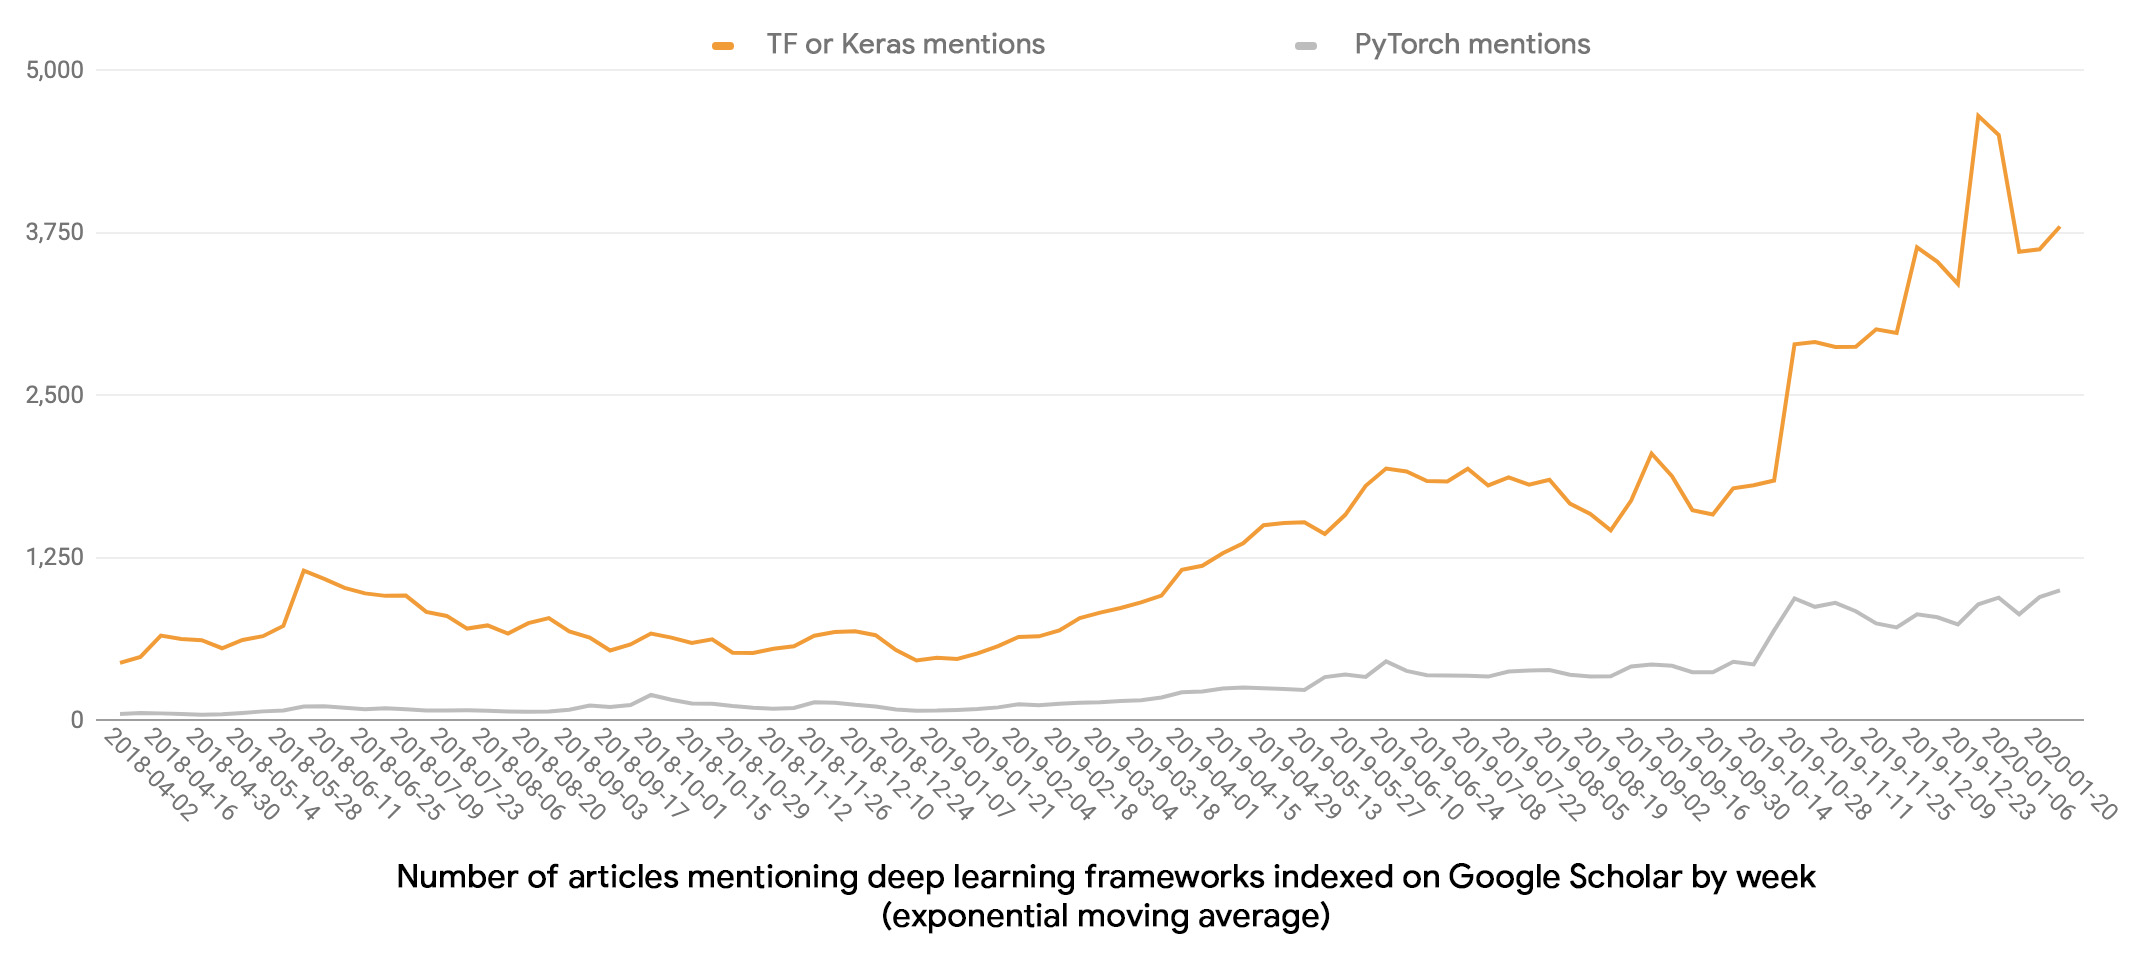
\includegraphics[width=1.1\textwidth]{figures/appendix/keras_vs_pytorch_mentions.jpeg}}
\caption{Chart highlighting the number of articles mentioning Keras and PyTorch. Figure downloaded from Keras website.}
\end{figure}

\begin{figure}[ht]
\centerline{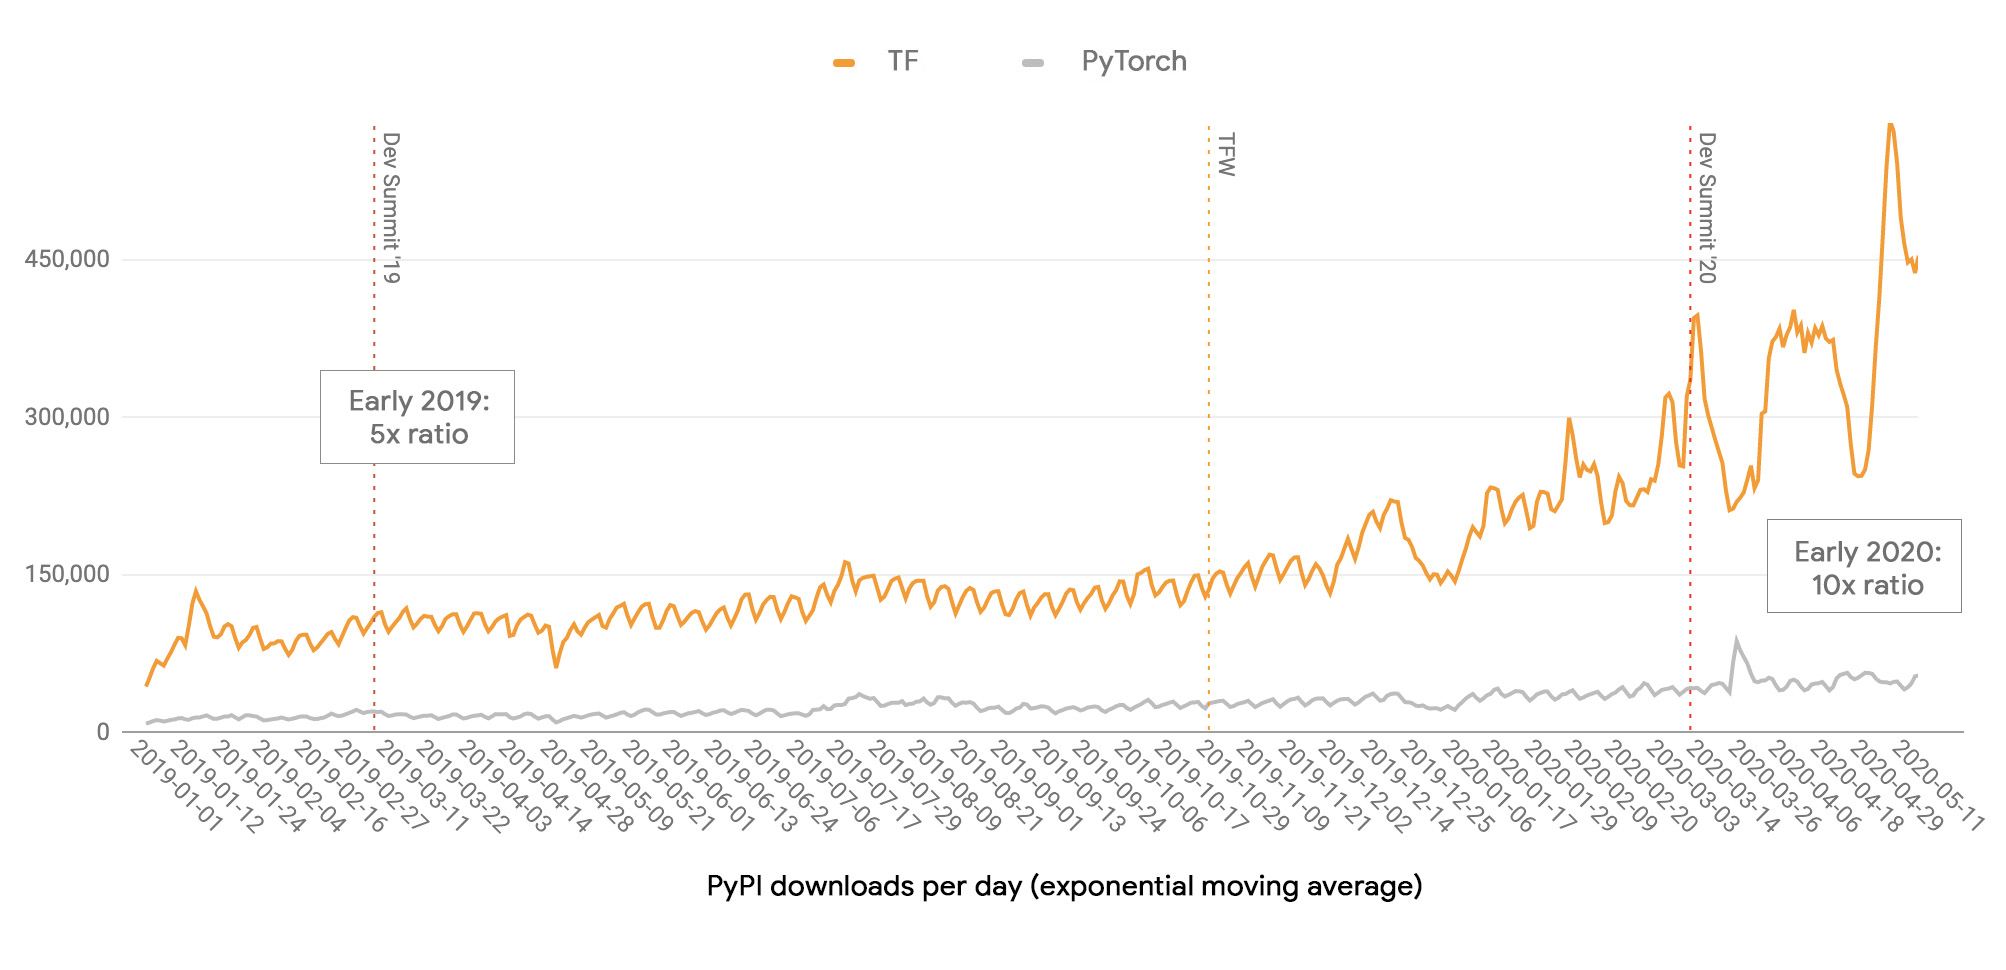
\includegraphics[width=1.1\textwidth]{figures/appendix/keras_vs_pytorch_downloads.jpg}}
\caption{Chart depicting the number of PyPI downloads for Keras and PyTorch. Figure downloaded from Keras website.}
\end{figure}
%%TC:endignore